\chapter{Dynamic Models: Part 2}\label{c:model2}

\section{Second-Order Model}
We will use \gls{second-order model} as shorthand for a linear, ordinary, time-invariant second-order differential equation of the form
\begin{equation} \label{e:second}
\ddot{y}(t) + 2 \zeta \omega_n \dot{y}(t) + \omega_n^2 = f(t)
\end{equation} 
where 
\begin{itemize}
\item $\ddot{y}(t)$ is the second derivative of $y(t)$ with respect to time,
\item $\dot{y}(t)$ is the first derivative of $y(t)$ with respect to time,
\item $y(t)$ is the solution to (\ref{e:second}),
\item $\zeta$ is the \gls{damping ratio},
\item $\omega_n$ is the \gls{undamped natural frequency} and
\item $f(t)$ is the input, or forcing function.
\end{itemize}
Just as with our first-order and static (zero-order) models, this model is an abstraction; it never has exactly the same behavior of a physical system, but it has been proven to be a useful approximation for the behavior of a variety of phenomena.  To understand the model we'll first present the solution to (\ref{e:second}) for a few types of input (forcing functions) and then work through some examples of cases where the model is a helpful abstraction of physical systems.

The intent of the following discussion is meant to be a summary and/or review of what you have seen in other courses (Differential Equations, System Dynamics, Feedback Controls, etc.).  The discussion should be sufficient for our purposes of modeling and measurement, but it is by no means an exhaustive treatment of analysis of second-order models or harmonic oscillator models.

Also, for now we are only interested in {\bf underdamped} and {\bf undamped} versions of the model (\ref{e:second}) where $0 \leq \zeta < 1.0$.  Another way to say this is that we are only interested in second-order models that have oscillations in their response.

\subsection{Example: Mass-Spring-Damper}
One type of physical system that has similar behavior to our second-order model is the mass-spring-damper system illustrated in Figure~\ref{f:msd2}.  (Actually, this system is still a bit of an abstraction; we rarely encounter applications that require a point mass attached to a mass-less spring.  The abstraction is meant to represent any physical system where there is inertia (mass, kinetic energy), a restoring force (spring, potential energy) and motion resistance (damper, energy dissipation).)
\begin{figure}[htb!]
\centerline{
{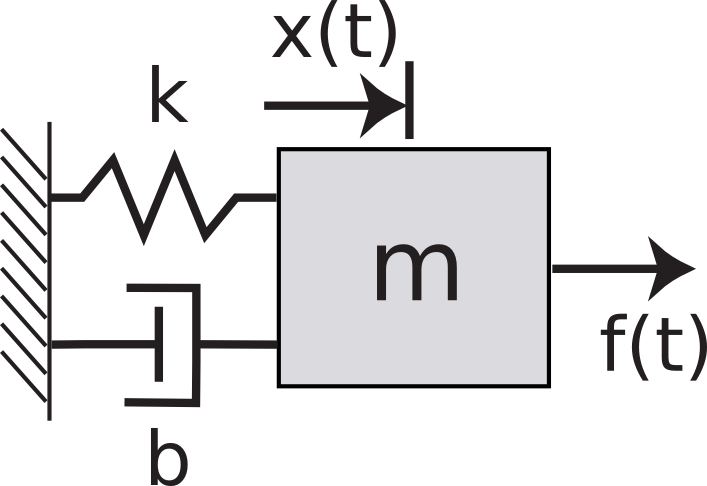
\includegraphics[width=0.4\textwidth]{msd_lower.png}}}
\caption{Sketch of a mass-spring-damper system.}
\label{f:msd2}
\end{figure}

If you draw a free-body-diagram of this system, you should be able to derive the second-order equation of motion
\begin{equation}\label{e:msd}
m \ddot{x}(t) + b \dot{x}(t) + k x(t) = f(t)
\end{equation}
where $m$ is the mass, $b$ is the linear damping coefficient, $k$ is the linear spring constant, $x(t)$ is the displacement of the mass and $f(t)$ is the input force.

\begin{ex}
Using (\ref{e:second}) and (\ref{e:msd}), derive expressions for the system parameters ($\omega_n$ and $\zeta$) in terms of the physical parameters ($m$, $b$, and $k$).  (Hint: Use physical units to check your answers.)
\end{ex}

\ifsolutions
\begin{soln}
\[ \omega_n = \sqrt{k/m} \; \; \; \unitfrac[]{rad}{s}\]
\[ \zeta = \frac{b}{2 \sqrt{mk}} \; \; \; \unitfrac[]{n}{a} \]
\end{soln}
\fi


\section{Free Response}\label{s:secondfree}
The free response for our model solution to the second-order model (\ref{e:second}) initial conditions, but no forcing function---also known as the homogeneous equation,
\begin{equation} \label{e:secondhomo}
\ddot{y}(t) + 2 \zeta \omega_n \dot{y}(t) + \omega_n^2 = 0
\end{equation} 
where the initial conditions at $t=0$ are
\begin{itemize}
\item $y(0) = y_o$ and 
\item $\dot{y}(0)=\dot{y}_o$.
\end{itemize}
Hopefully you've been convinced that this type of differential equation is straightforward to solve (in theory), and we can present (without derivation) that the solution to this equation is the function
\begin{equation} \label{e:secondfree}
y(t) = C \left(e^{-\zeta \omega_n t}\right) \left( \cos(\omega_d t - \phi) \right).
\end{equation}
where
\begin{eqnarray}\
\omega_d & = & \omega_n \sqrt{1-\zeta^2} \label{e:damped} \\
C & = & \sqrt{ y_o^2 + \left( \frac{\dot{y}_o+\zeta\omega_n y_o}{\omega_d} \right)^2 } \;\; \mathrm{and}\label{e:C} \\
\tan(\phi) & = & \frac{\dot{y}_o+\zeta \omega_n y_o}{\omega_d y_o}. \label{e:phi}
\end{eqnarray}

The free response (\ref{e:secondfree}) is the key part of all this.  There are many systems that behave in this general way with a decaying oscillatory response.  To illustrate this we can annotate the equation to highlight the three parts of the solution:
\begin{equation} \label{e:secondfree_annote}
y(t) = \underbrace{C}_\text{constant} 
\underbrace{\left(e^{-\zeta \omega_n t}\right)}_\text{exponential decay}
\underbrace{\left( \cos(\omega_d t - \phi) \right)}_\text{oscillation}.
\end{equation}
One important detail is that there are two slightly different ``natural frequencies'' to keep track of.  The \gls{undamped natural frequency} ($\omega_n$) is the parameter we saw in the system model and which is included in the exponential decay component of (\ref{e:secondfree_annote}).  The \gls{damped natural frequency} ($\omega_d$) is the frequency of oscillation, the angular frequency inside the $\cos$ term of (\ref{e:secondfree_annote}).  The relation between the two values is given in (\ref{e:damped}).  For small values of $\zeta$, so called ``lightly damped systems'', there is little difference between the two values.

Another way to ``see'' this solution is to graph the time response.  The short MATLAB script in Listing~\ref{l:secondfree} generates Figure~\ref{f:secondfree}.  This figure illustrates the key characteristics of a second order free response:
\begin{enumerate}
\item the system oscillates at a constant frequency (the $\cos(\omega_d t)$ term) and
\item the amplitude of the oscillations decays exponentially over time (the $e^{=\zeta \omega_n t}$ term).
\end{enumerate}
%\lstinputlisting[style=myMatStyle,
%caption={Script for plotting the free response of a second-order model (\verb+second_order_free.m+).},
%label={l:second_free}]
%{./code/second_order_free.m}

\lstinputlisting[style=myMatStyle,
caption={Script for plotting the free response of a second-order model.},
label={l:secondfree}]
{./code/second_order_free.m}


\begin{figure}[hbt]
\centering
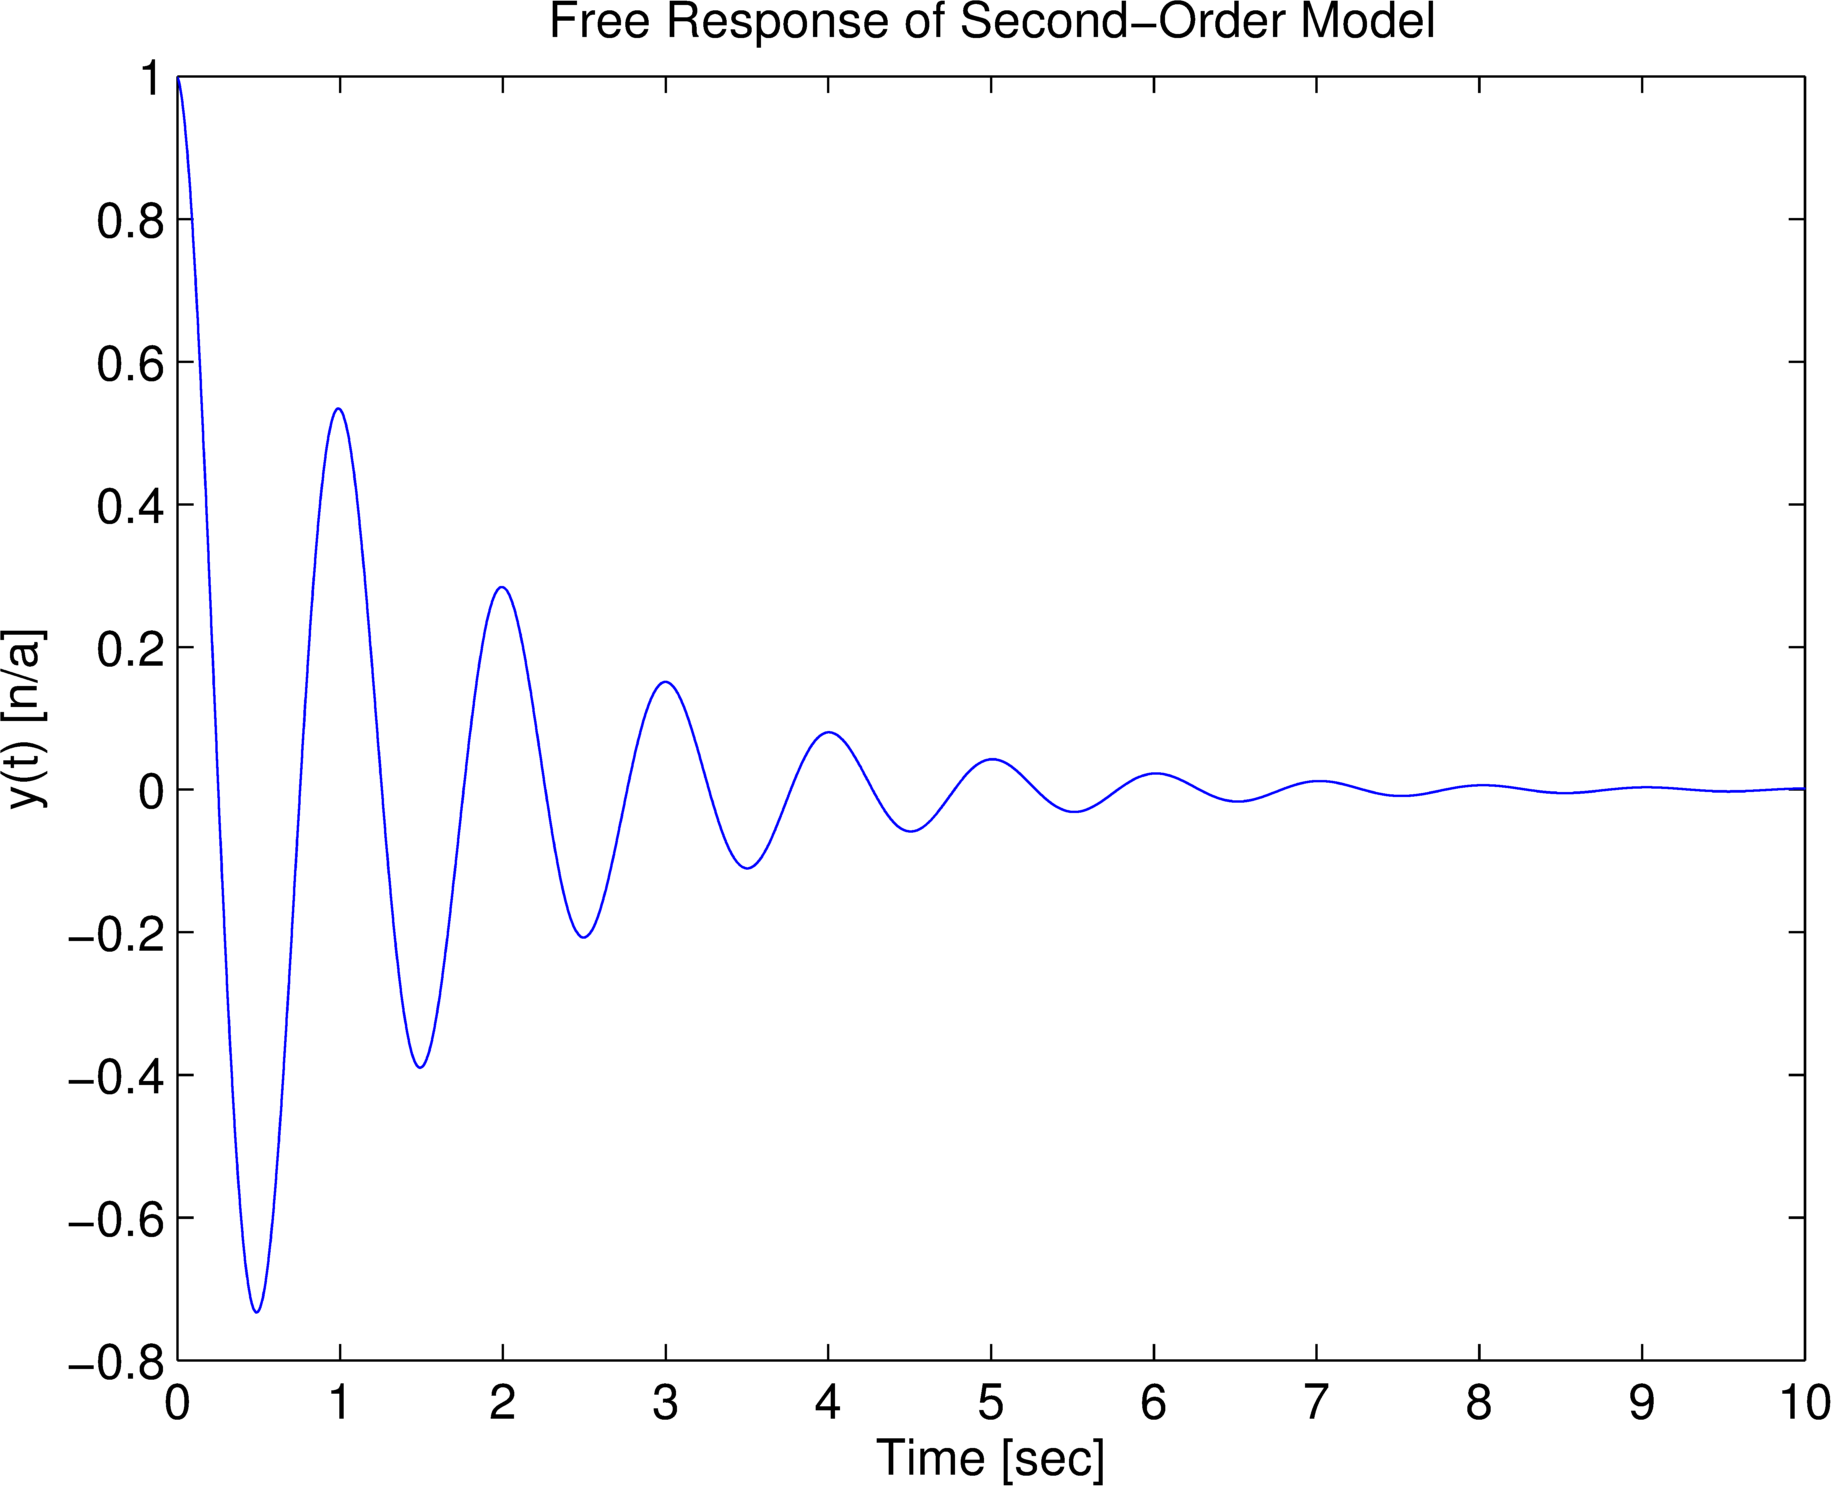
\includegraphics[width=\FigWidth\textwidth]{second_free.png}
\caption{Graph of the free response (\ref{e:stepresp}) with $\omega_n= \unit[1]{Hz}$, $\zeta=0.1$ (10\%) and $y(t=0)=1$.}
\label{f:secondfree}
\end{figure}

\begin{ex}
There is a mistake in Listing~\ref{l:secondfree} which attempted to display the solution for the case where there is only a ``displacement'' initial condition: i.e., $y(0)=y_o$ and $\dot{y}(0)=0$.  The mistake is that the solution in the code uses the values $C=y_o$ and $\phi=0$ which are not correct (but they are close). 
\begin{itemize}
\item Derive expressions for the constants $C$ and $\phi$ based on the initial conditions $y(0)=y_o$ and $\dot{y}(0)=0$.
\item Copy the script in Listing~\ref{l:secondfree} and create the graph shown in Figure~\ref{f:secondfree}.
\item Correct the script in Listing~\ref{l:secondfree} and plot a second curve, on the same axes, with the corrected solution for $y_o=1$.  
  \begin{itemize}
  \item Include your MATLAB script with your solution.
  \item Include your graph as a properly formatted figure.
  \end{itemize}
\end{itemize}
The error is simply in the calculation of $C$ and $\phi$; the structure of the script in Listing~\ref{l:secondfree} should work just fine.
\end{ex}

\ifsolutions
\begin{soln}
\[ C = \sqrt{\frac{y_o}{1-\zeta^2}} \]
\[ \tan\phi = \frac{\zeta}{\sqrt{1-\zeta^2}} \]
or 
\[ \phi = \arctan\left(\frac{\zeta}{\sqrt{1-\zeta^2}}\right) \]

See Figure~\ref{f:secondfreesoln}.

\begin{figure}[hbt]
\centering
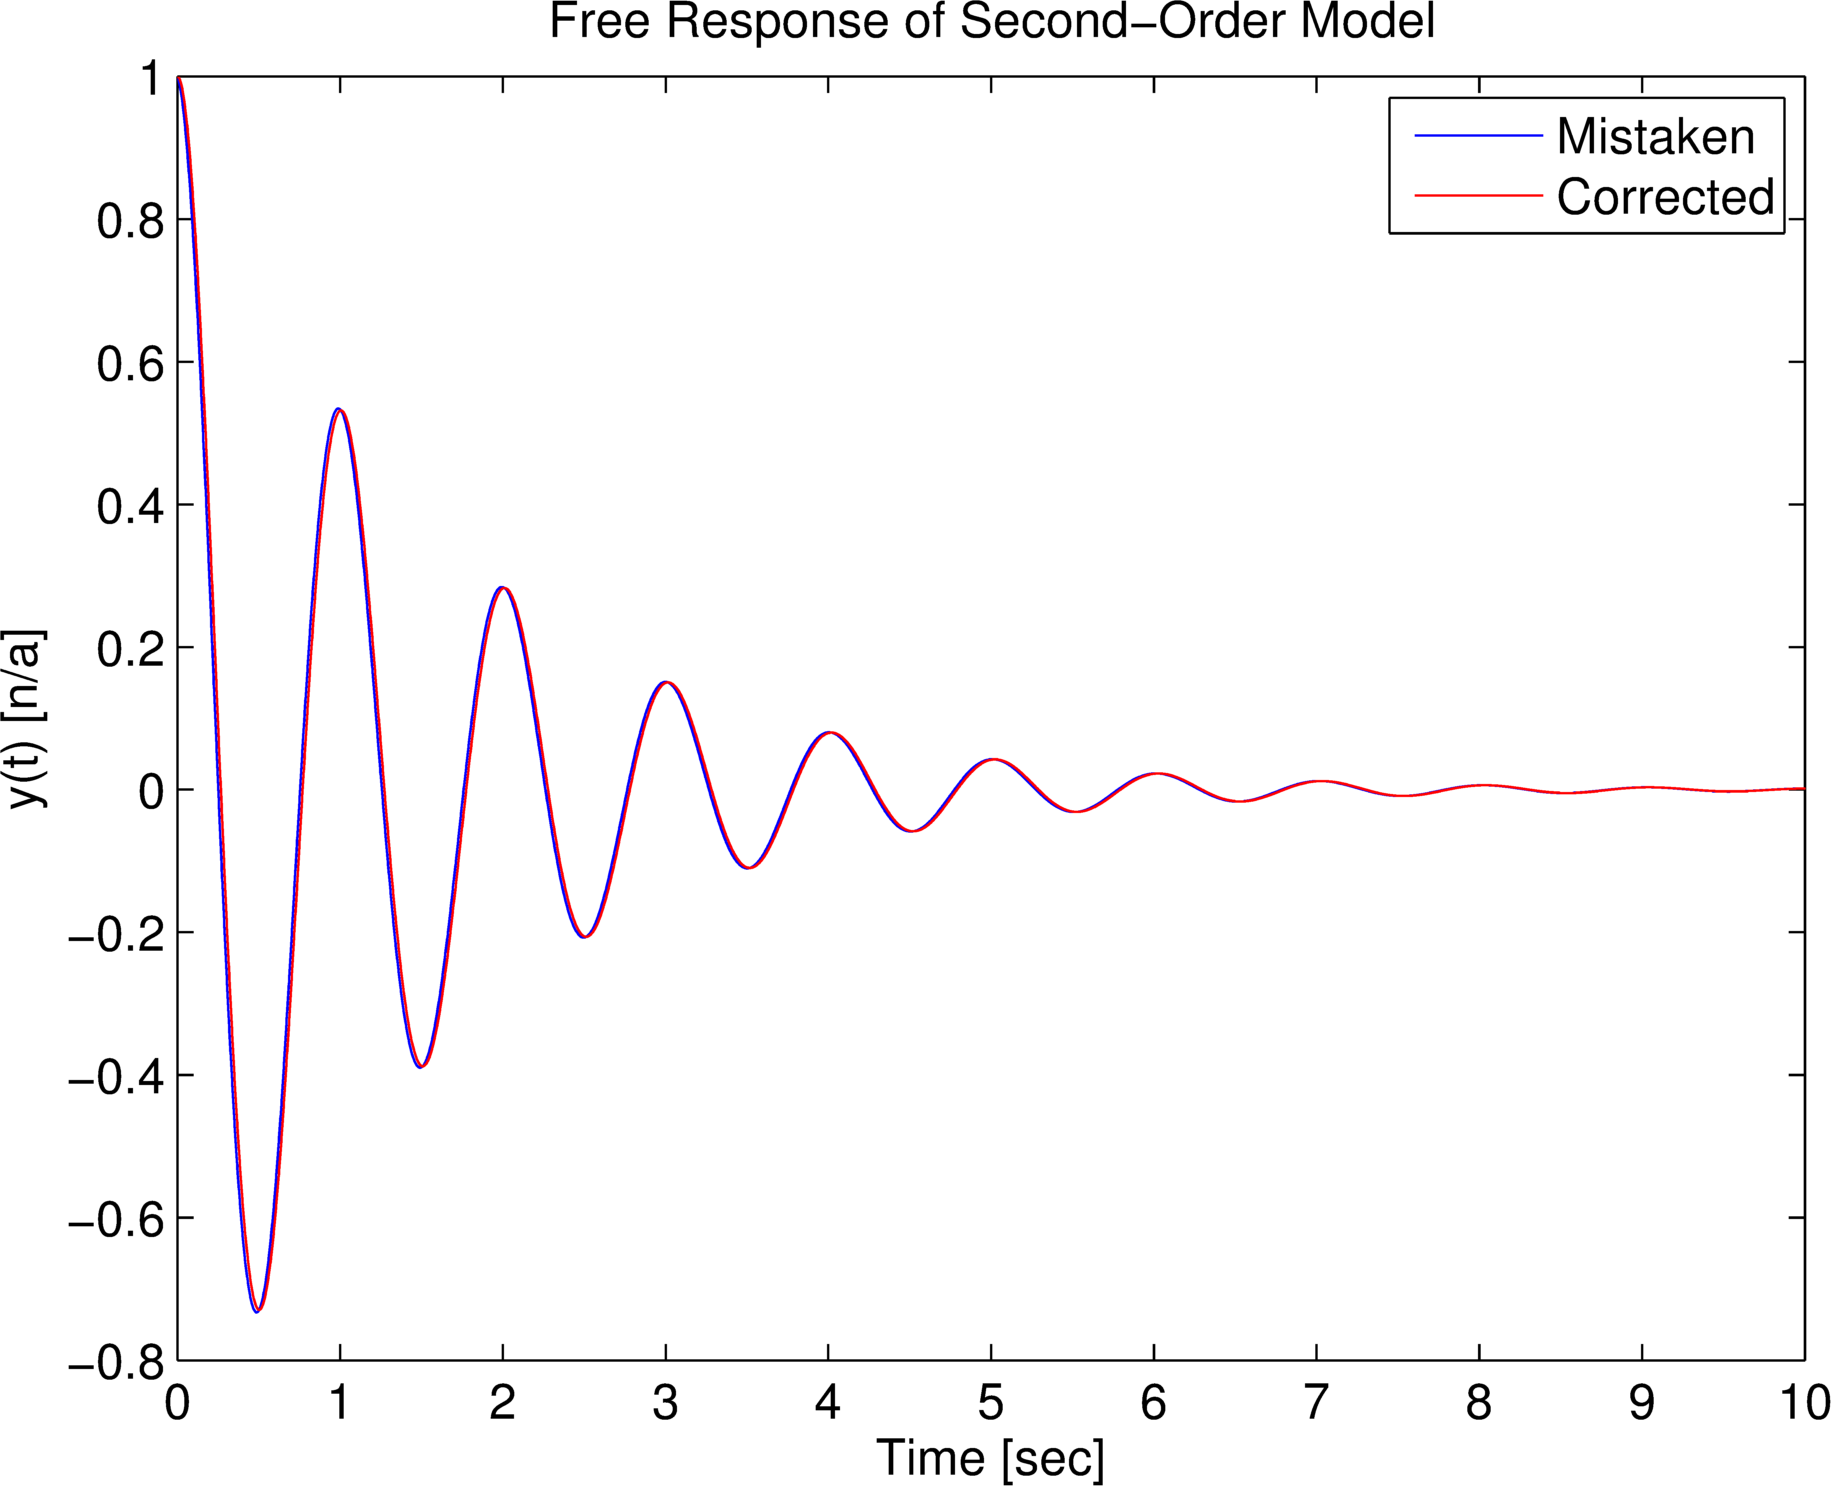
\includegraphics[width=\FigWidth\textwidth]{second_free_soln.png}
\caption{Graphs of the original mistaken free response and the corrected free response.}
\label{f:secondfreesoln}
\end{figure}
\end{soln}
\fi

\begin{ex}
Consider the effect of the damping ratio ($\zeta$) on the shape of free response.  Using Listing~\ref{l:secondfree} as a starting point, use MATLAB to create a single graph for the free response with the initial conditions $y(0)=1$ and $\dot{y}(0)=0$.  On a single set of axes, plot the response for systems with the following values for the damping ratio: $\zeta=\{0.0, 0.01 , 0.1, 0.5, 0.9\}$.  Use a legend to declare which curve is associated with each value of $\zeta$.  Submit this single graph as an appropriately formatted figure with a short description of what you observe about the effect of changing $\zeta$.
\end{ex}

\ifsolutions
\begin{soln}
See Figure~\ref{f:secondfreezetas}
\begin{figure}[hbt]
\centering
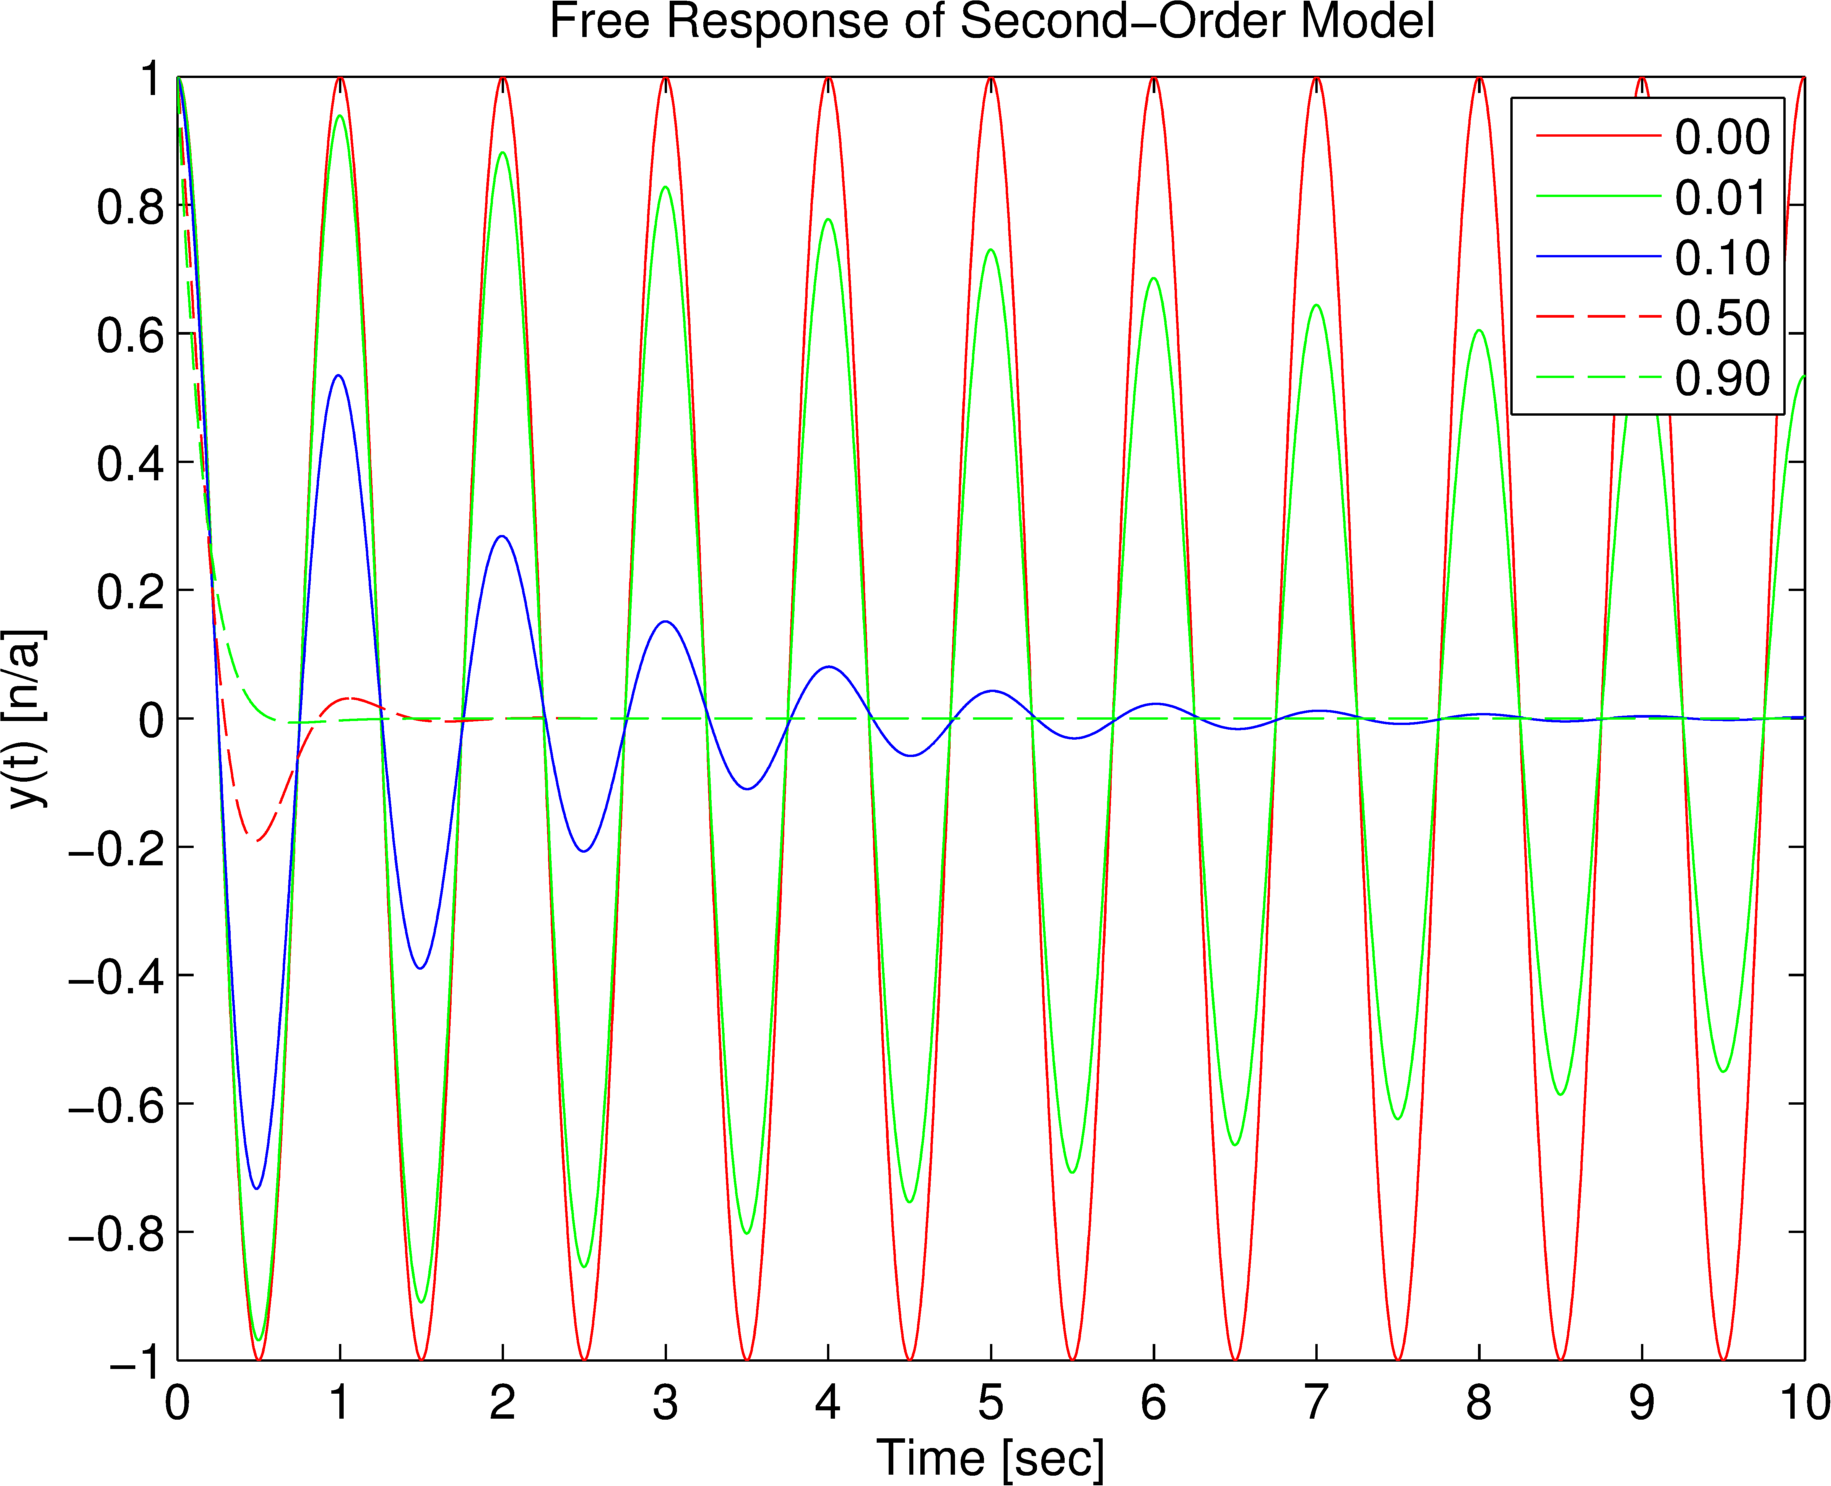
\includegraphics[width=\FigWidth\textwidth]{free_zetas.png}
\caption{}
\label{f:secondfreezetas}
\end{figure}

\end{soln}
\fi

\begin{ex}
Consider the model's free response to velocity-only initial conditions---$y(0)=0$ and $\dot{y}(0)=v_o$.
\begin{itemize}
\item Derive expressions for the constants $C$ and $\phi$ based on these initial conditions.
\item Substitute your expressions into the response (\ref{e:secondfree}) and write a simplified equation for the response.  (Hint: $\cos\left(u-\frac{\pi}{2}\right) = \sin(u)$.)
\item Using MATLAB, create a figure the graphs the response ($y(t)$) to this initial condition.
\end{itemize}
\end{ex}


\begin{ex}
Given a damping ratio of $\zeta=0.01$ (1\% damping), write and expression for the damped natural frequency as a function of the undamped natural frequency.  \\
Repeat the exercise for a 10\% damping.
\end{ex}

\section{Example: Cantilevered Beam}
Another physical system that has a response that can be approximated by our second-order model is a cantilevered beam.  Imagine a yardstick fixed on one end.  When the free end is subject to a displacement (the initial condition) and then released, the tip will oscillate.  A cantilevered beam, unlike our lumped mass system in Figure~\ref{f:msd2}, is a continuous system, but for now we'll approximate it by examining the first natural frequency.  

\subsection{First-Mode of Cantilevered Beam}
The first natural frequency of a uniform cantilevered beam, Figure~\ref{f:blevins}, can be estimated by using classical beam theory.
\begin{figure}[htb!]
\centerline{
{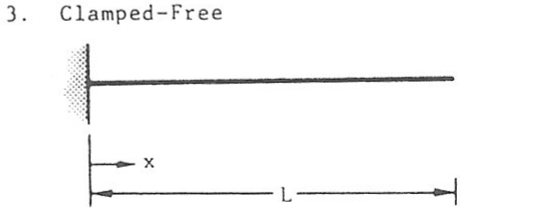
\includegraphics[width=0.4\textwidth]{blevins_beam.png}}}
\caption{Image of a cantilevered beam model.  From ``Formulas for Natural Frequency and Mode Shape'' by R. D. Blevins.}
\label{f:blevins}
\end{figure}
The resulting expression for the first natural frequency, in \unitfrac[]{rad}{s}, is
\begin{equation}\label{e:blevins}
\omega_n = \frac{(1.875)^2}{L^2} \sqrt{\left( \frac{EI}{\rho} \right)}
\end{equation}
where $\rho$ is the mass per unit length of the beam, $E$ is the modulus of elasticity of the beam material, $I$ is the area moment of inertia of the beam and $L$ is the length of the beam. 

\subsection{First-Mode of Cantilevered Beam with Added Mass}
Similarly, it is possible to predict the natural frequency of a uniform cantilevered beam with a point-mass at the free end of the beam as illustrated in Figure~\ref{f:blevinsmass}.
\begin{figure}[htb!]
\centerline{
{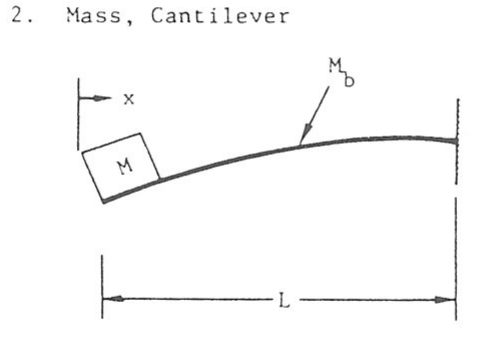
\includegraphics[width=0.4\textwidth]{blevins_beam_mass.png}}}
\caption{Image of a cantilevered beam with point mass model from ``Formulas for Natural Frequency and Mode Shape'' by R. D. Blevins.}
\label{f:blevinsmass}
\end{figure}
The first natural frequency for this model is
\begin{equation}\label{e:blevinsmass}
\omega_n = \sqrt{ \frac{3 E I}{L^3 (M+0.24 M_b)}}
\end{equation}
where $M$ is the point mass at the free end of the beam and $M_b$ is the total mass of the beam.

Notice that both predicted natural frequencies (\ref{e:blevins}) and (\ref{e:blevinsmass}) have the general from of $\omega_n = \sqrt{K/M}$ where $K$ is the ``stiffness'' of the system and $M$ is the ``mass'' of the system.


\begin{ex}
Given a uniform cantilevered beam with the following properties:
\begin{itemize}
\item Length = \unit[0.5]{m}
\item Width = \unit[2.54]{cm}
\item Thickness = \unit[1.59]{mm}
\item Modulus of Elasticity ($E$) = \unit[68.9]{GPa}
\item Density = \unitfrac[2.70]{g}{cm$^3$}
\end{itemize}
Predict the undamped natural frequency in \unit[]{rad}{s} and \unit[]{Hz}.
\end{ex}

\begin{ex}
Given the uniform cantilevered beam described in the previous example, and a damping ratio of $\zeta=0.02$ (2\% damping)...
\begin{itemize}
\item Write an expression for a mathematical model of the form in (\ref{e:second}) to describe the system.
\item Using MATLAB, produce a graph that predicts the response of the tip of the cantilevered beam to an initial displacement of \unit[1.0]{cm}.
\end{itemize}
\end{ex}

\section{Measuring Second-Order Response}
For physical systems that exhibit oscillatory response we can ``fit'' a second-order response to the system measurements to estimate the system parameters ($\omega_n$ and $\zeta$) based on the measured response.  In other words, consider that you measure the time response of a system (e.g., a cantilevered beam, a RLC circuit, etc.) and you observe that the behavior looks something like Figure~\ref{f:secondfreeresp}.  How can you estimate the natural frequency and damping ratio associated with such a response?

\begin{figure}[h!bt]
\centerline{
{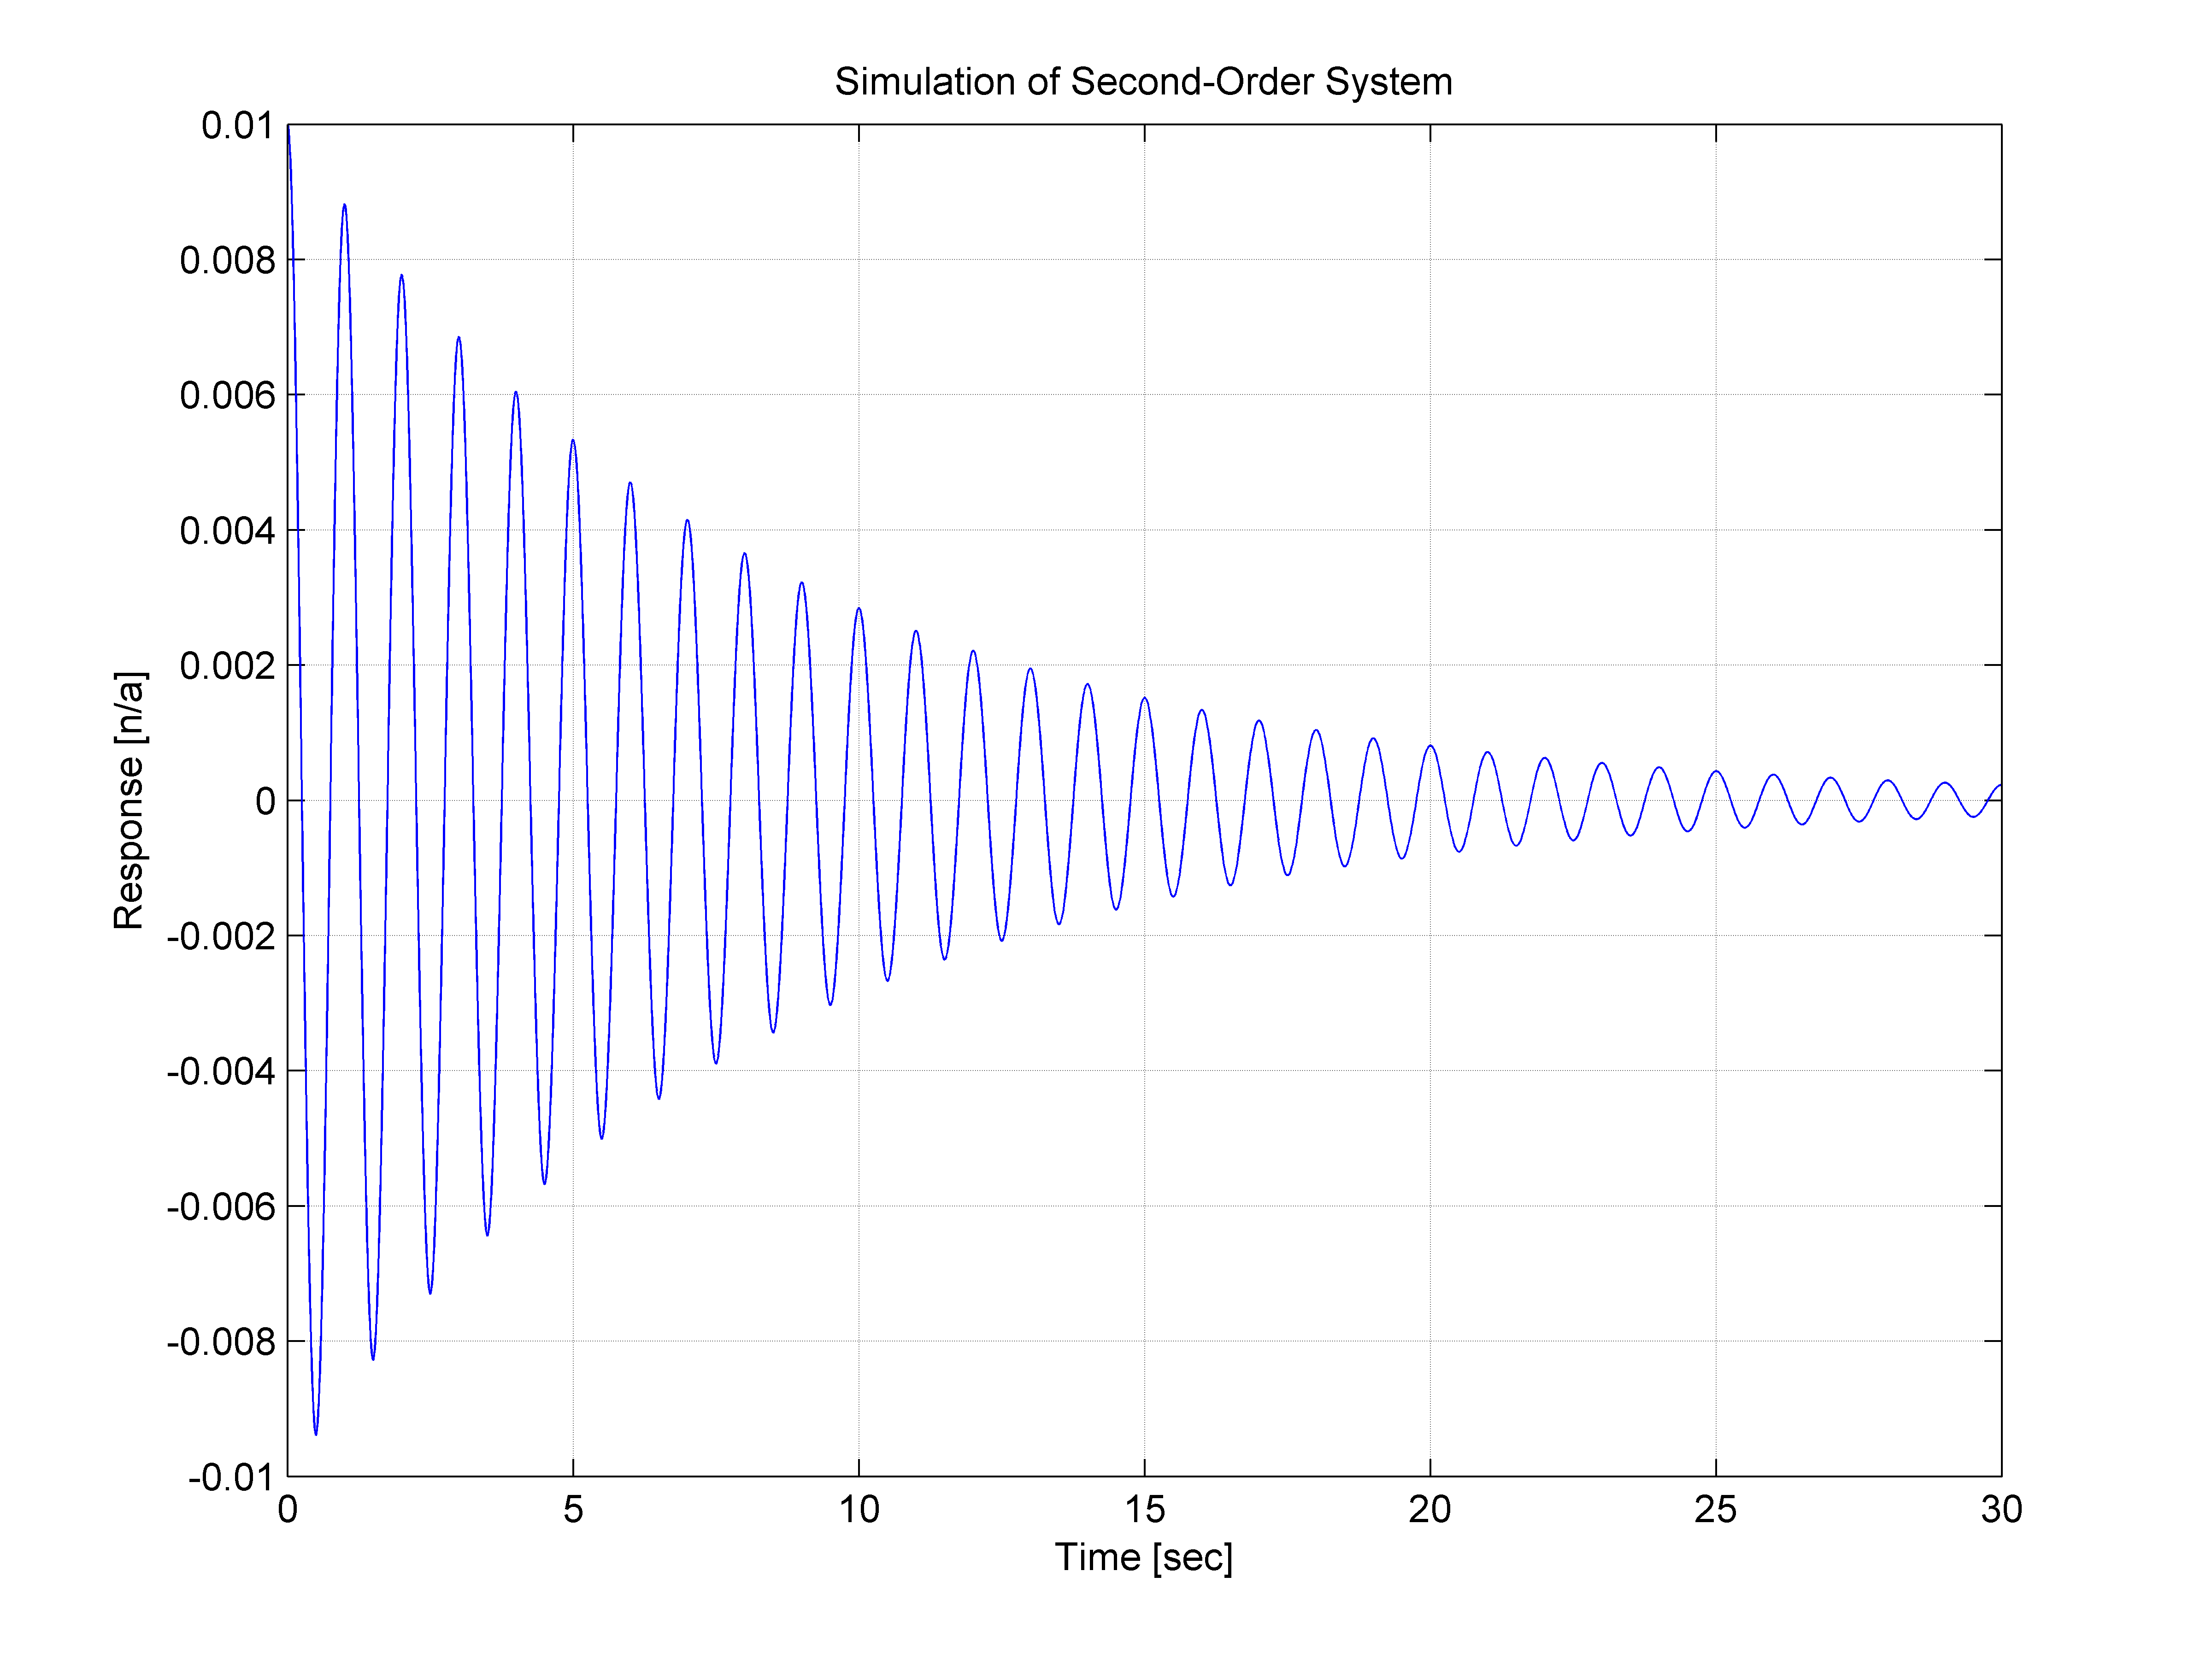
\includegraphics[width=0.6\textwidth]{second_order_grid.png}}}
\caption{Illustration of the free-response of a second-order system.  The response shows the analytical solution for $y(t)$.}
\label{f:secondfreeresp}
\end{figure}

\subsection{Measuring Frequency}
It may be obvious, but if for no other reason than to get the units (\unit[]{Hz} and \unitfrac[]{rad}{s}) it is worth spending a little time discussing how to measure the frequency of oscillation from a measured response.  Since our measurements are of the {\bf time} response, we will need to start by estimating the period of oscillation, the time it takes for one cycle of oscillation.  We could do this by measuring the time between two adjacent peaks in the response, but a better way is to measure the elapsed time ($\Delta t$) between two peaks (or troughs, or zero-crossings) of the response and the number of cycles ($n$) as illustrated in Figure~\ref{f:secondtime}.
\begin{figure}[h!bt]
\centerline{
{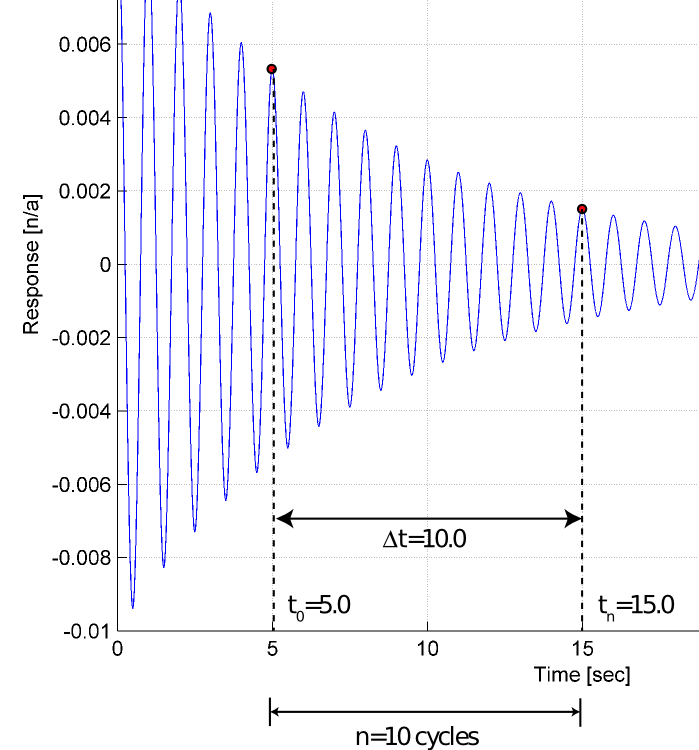
\includegraphics[width=0.6\textwidth]{second_order_grid_time_only_annote_crop.png}}}
\caption{Illustration of measuring the period of oscillation.}
\label{f:secondtime}
\end{figure}
Then we can estimate the average period of oscillation as
\begin{equation}
T = \frac{t_n-t_o}{n}=\frac{\Delta t}{n}=\frac{\unit[10.0]{s}}{\unit[10]{cycles}} = \unitfrac[1.0]{s}{cycle}.
\end{equation}
The corresponding frequency of oscillation ($f_d$ (in Hz)) is the reciprocal of the period---
\begin{equation}
f_d = \frac{1}{T} = \frac{1}{\unitfrac[1.0]{s}{cycle}} = \unitfrac[1.0]{cycles}{s} = \unit[1.0]{Hz}.
\end{equation}
The last step is convert the units of this frequency from Hz to \unitfrac[]{rad}{s} with the expression
\begin{equation}
\omega_d = f_d (2 \pi) = \unitfrac[1.0]{cycles}{s} (\unitfrac[2 \pi]{rad}{cycle}) = \unitfrac[6.28]{rad}{s}.
\end{equation}
It is important to notice that what we have estimated here is the {\bf damped} natural frequency ($\omega_d$), not the undamped natural frequency ($\omega_n$).  Again, the relationship between these two quantities is
\begin{equation}
\omega_n = \frac{\omega_d}{\sqrt{1-\zeta^2}}.
\end{equation}
To estimate $\omega_n$ we'll need to know (to estimate) the damping ratio ($\zeta$).

\subsection{Measuring the Damping Ratio Via Logarithmic Decrement Method}

The logarithmic decrement method is a technique to empirically identify the damping ratio ($\zeta$) of a second-order underdamped model.  The method is based on the characteristic time response of the model.  The time response can be either the response to a step input or the free-response to a non-zero initial condition.  The free-response to an initial condition is given in your textbook as
\begin{equation}
y_h(t)=C e^{-\zeta\omega_nt}\sin\left(\omega_dt+\phi\right) 
\end{equation}
where $\omega_n$ is the undamped natural frequency of the system and $\omega_d=\omega_n\sqrt{1-\zeta^2}$ is the damped natural frequency.  The two constants $C$ and $\phi$ are determined from the initial conditions.

To estimate the damping ratio can be estimated in the following way.  First plot the response $y(t)$ as a function of time.  Choose two peaks of the oscillatory response $y_0$ and $y_n$ where $y_0$ is the larger value that happens earlier in time.  Calculate the logarithmic decrement ($\delta$) as
\[ \delta = \frac{1}{n}\ln\left(\frac{y_0}{y_n}\right) \]
where $n$ is the number of cycles between $y_0$ and $y_n$.
Finally calculate the damping ratio as
\[ \zeta = \frac{1}{\sqrt{1+\left(\frac{2\pi}{\delta}\right)^2}} \]

\subsubsection{Example}
Figure \ref{f:secondfreeresp} illustrates the free response of a second-order model to an initial condition of $y(0)=0.01$ and $\dot{y}(0)=0$.  The undamped natural frequency is \unitfrac[$2 \pi$]{rad}{s}.

To calculate the logarithmic decrement we need to select two peaks from the response as shown in Figure~\ref{f:resp2}\footnote{The MATLAB function \texttt{ginput()} is handy for selecting the values from a figure window.}. These selected values, along with the equations above, result in $\delta=0.124$ and $\zeta=0.0198$.  This estimate is quite close to the value of 0.02 which was used to generate the example.

\begin{figure}[h!bt]
\centerline{
{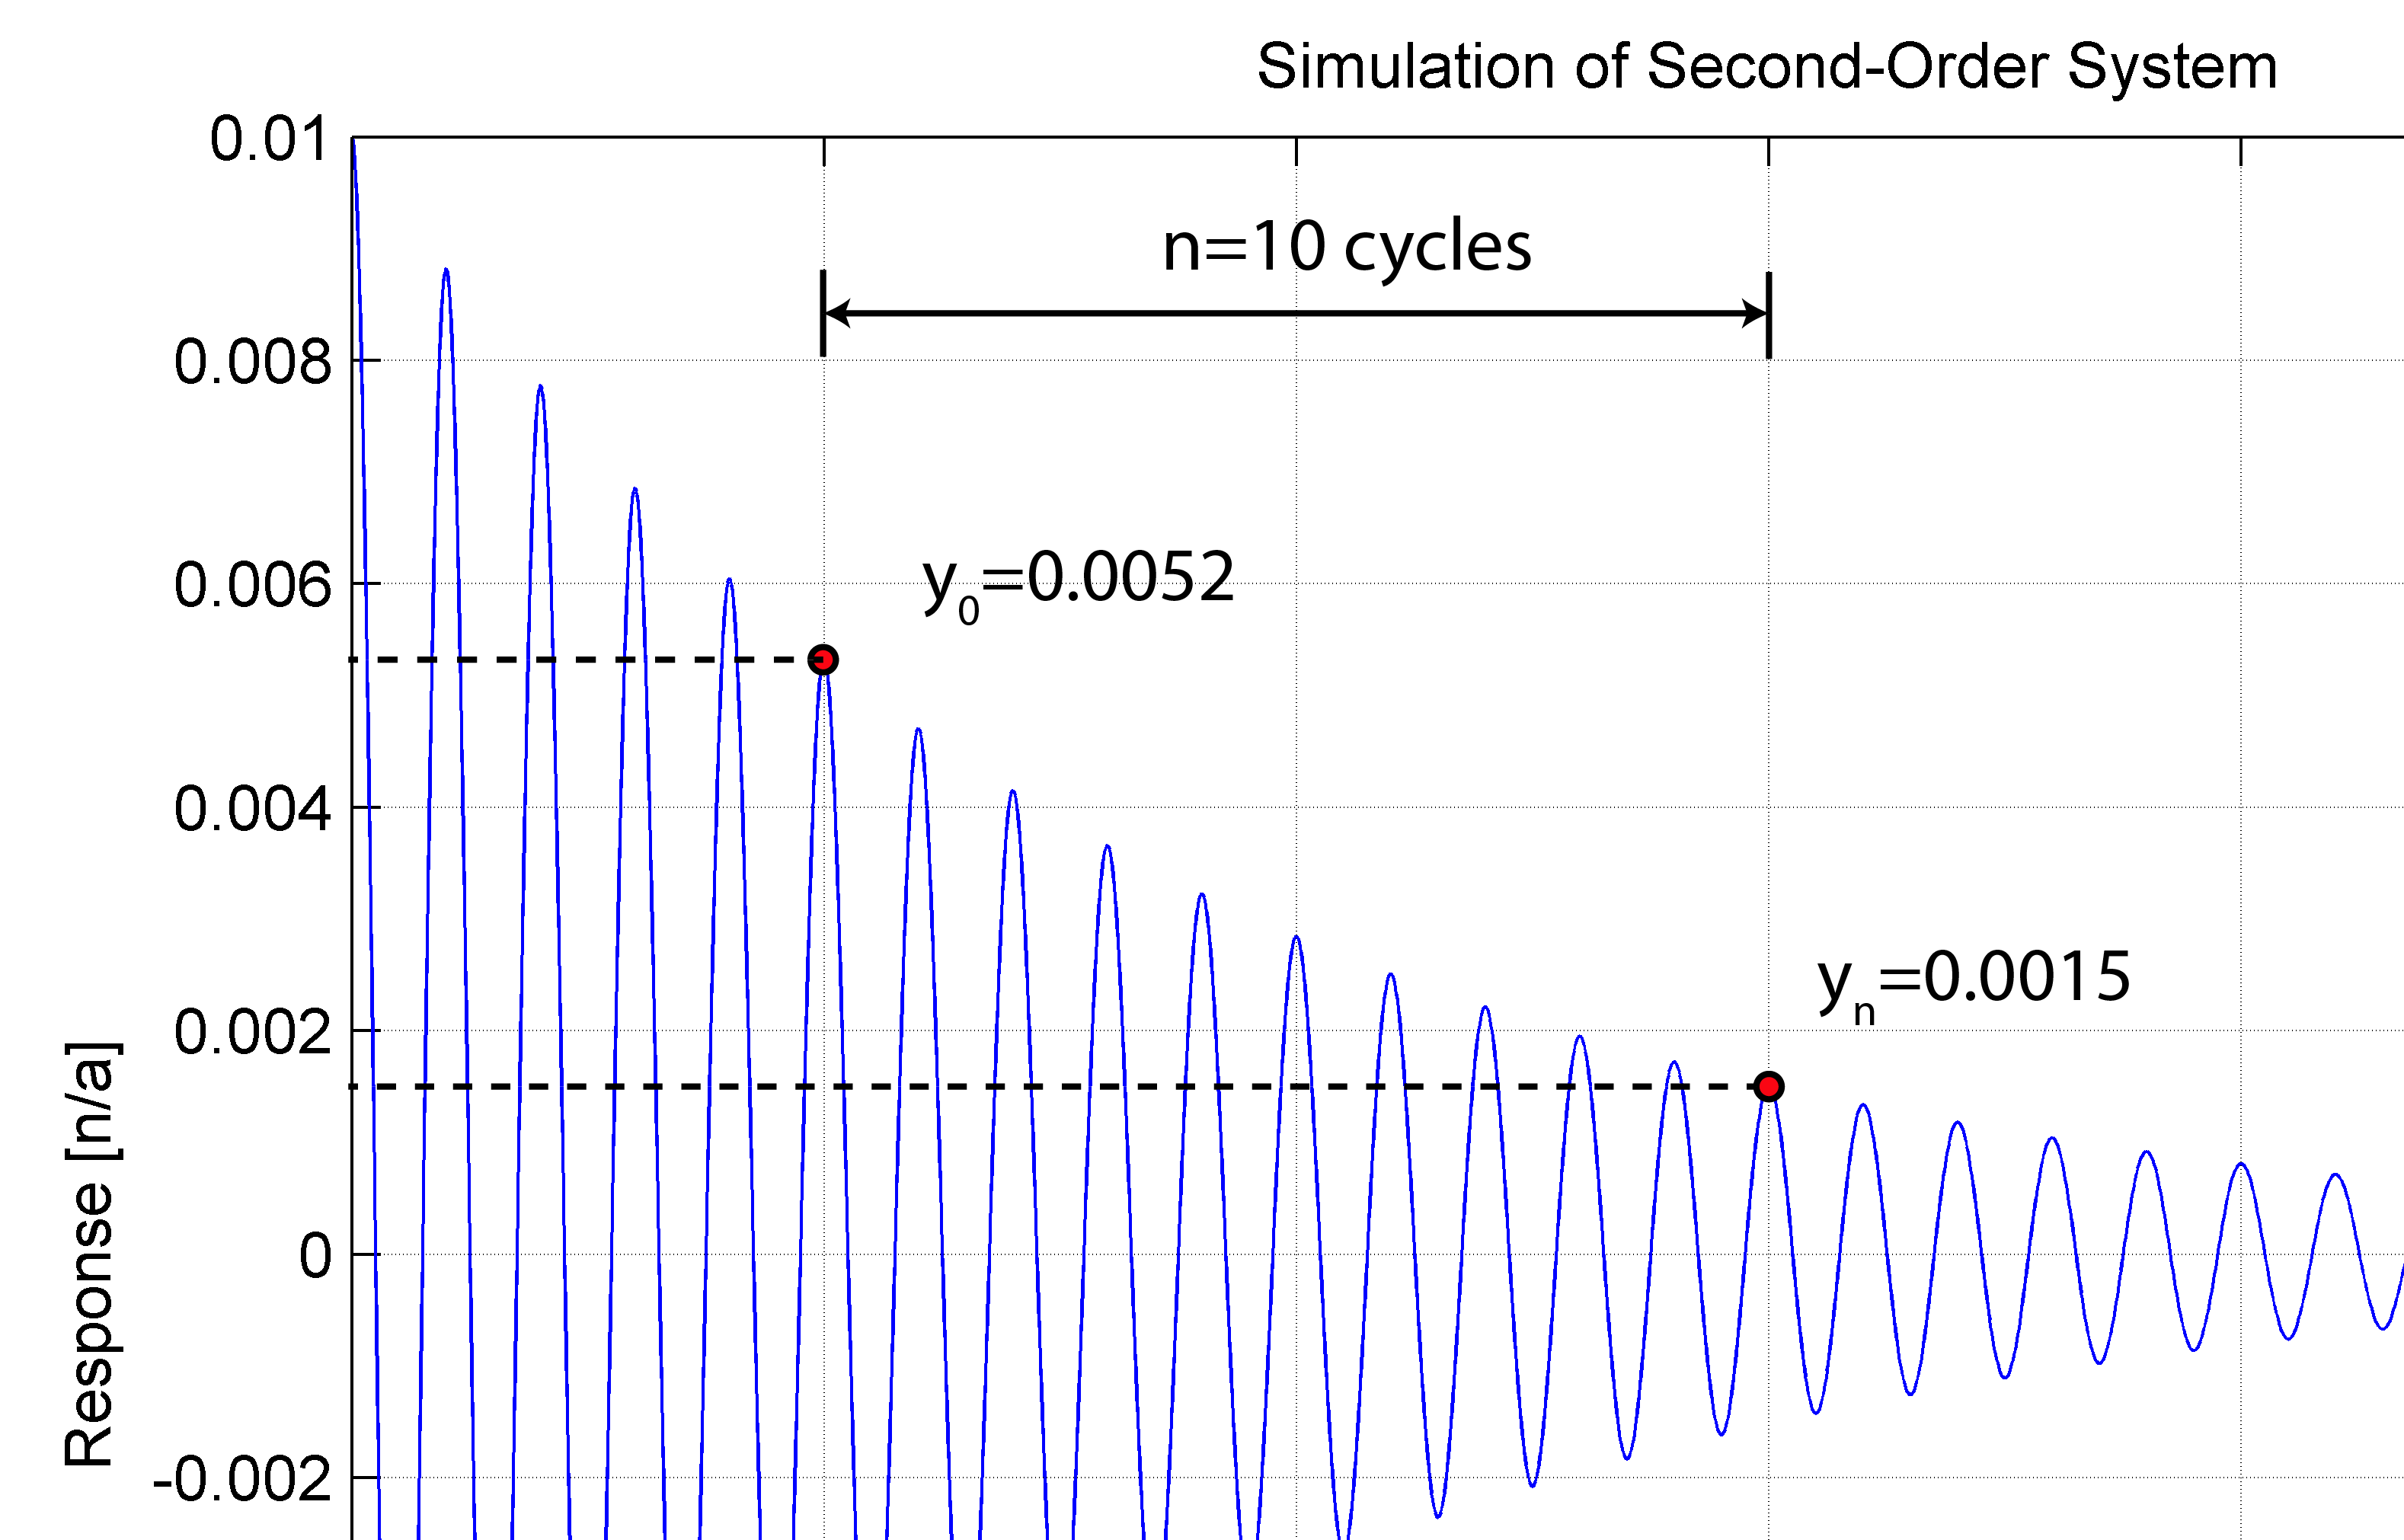
\includegraphics[width=0.6\textwidth]{second_order_grid_annote_crop.png}}}
\caption{The added annotation illustrates the selection of ``peaks'' in the response to initiate the logarithmic decrement process.}
\label{f:resp2}
\end{figure}

%\afterpage{\clearpage}

\subsubsection{Why It Works}
The logarithmic decrement method is based on fitting a curve to the data.  In this case the curve (the model) is the exponential amplitude of the second-order response
\begin{equation}
y_{env}(t)=C e^{-\zeta\omega_nt}
\label{e:env}
\end{equation}
This function is superimposed on the response in Figure~\ref{f:env}.
\begin{figure}[h!bt]
\centerline{
{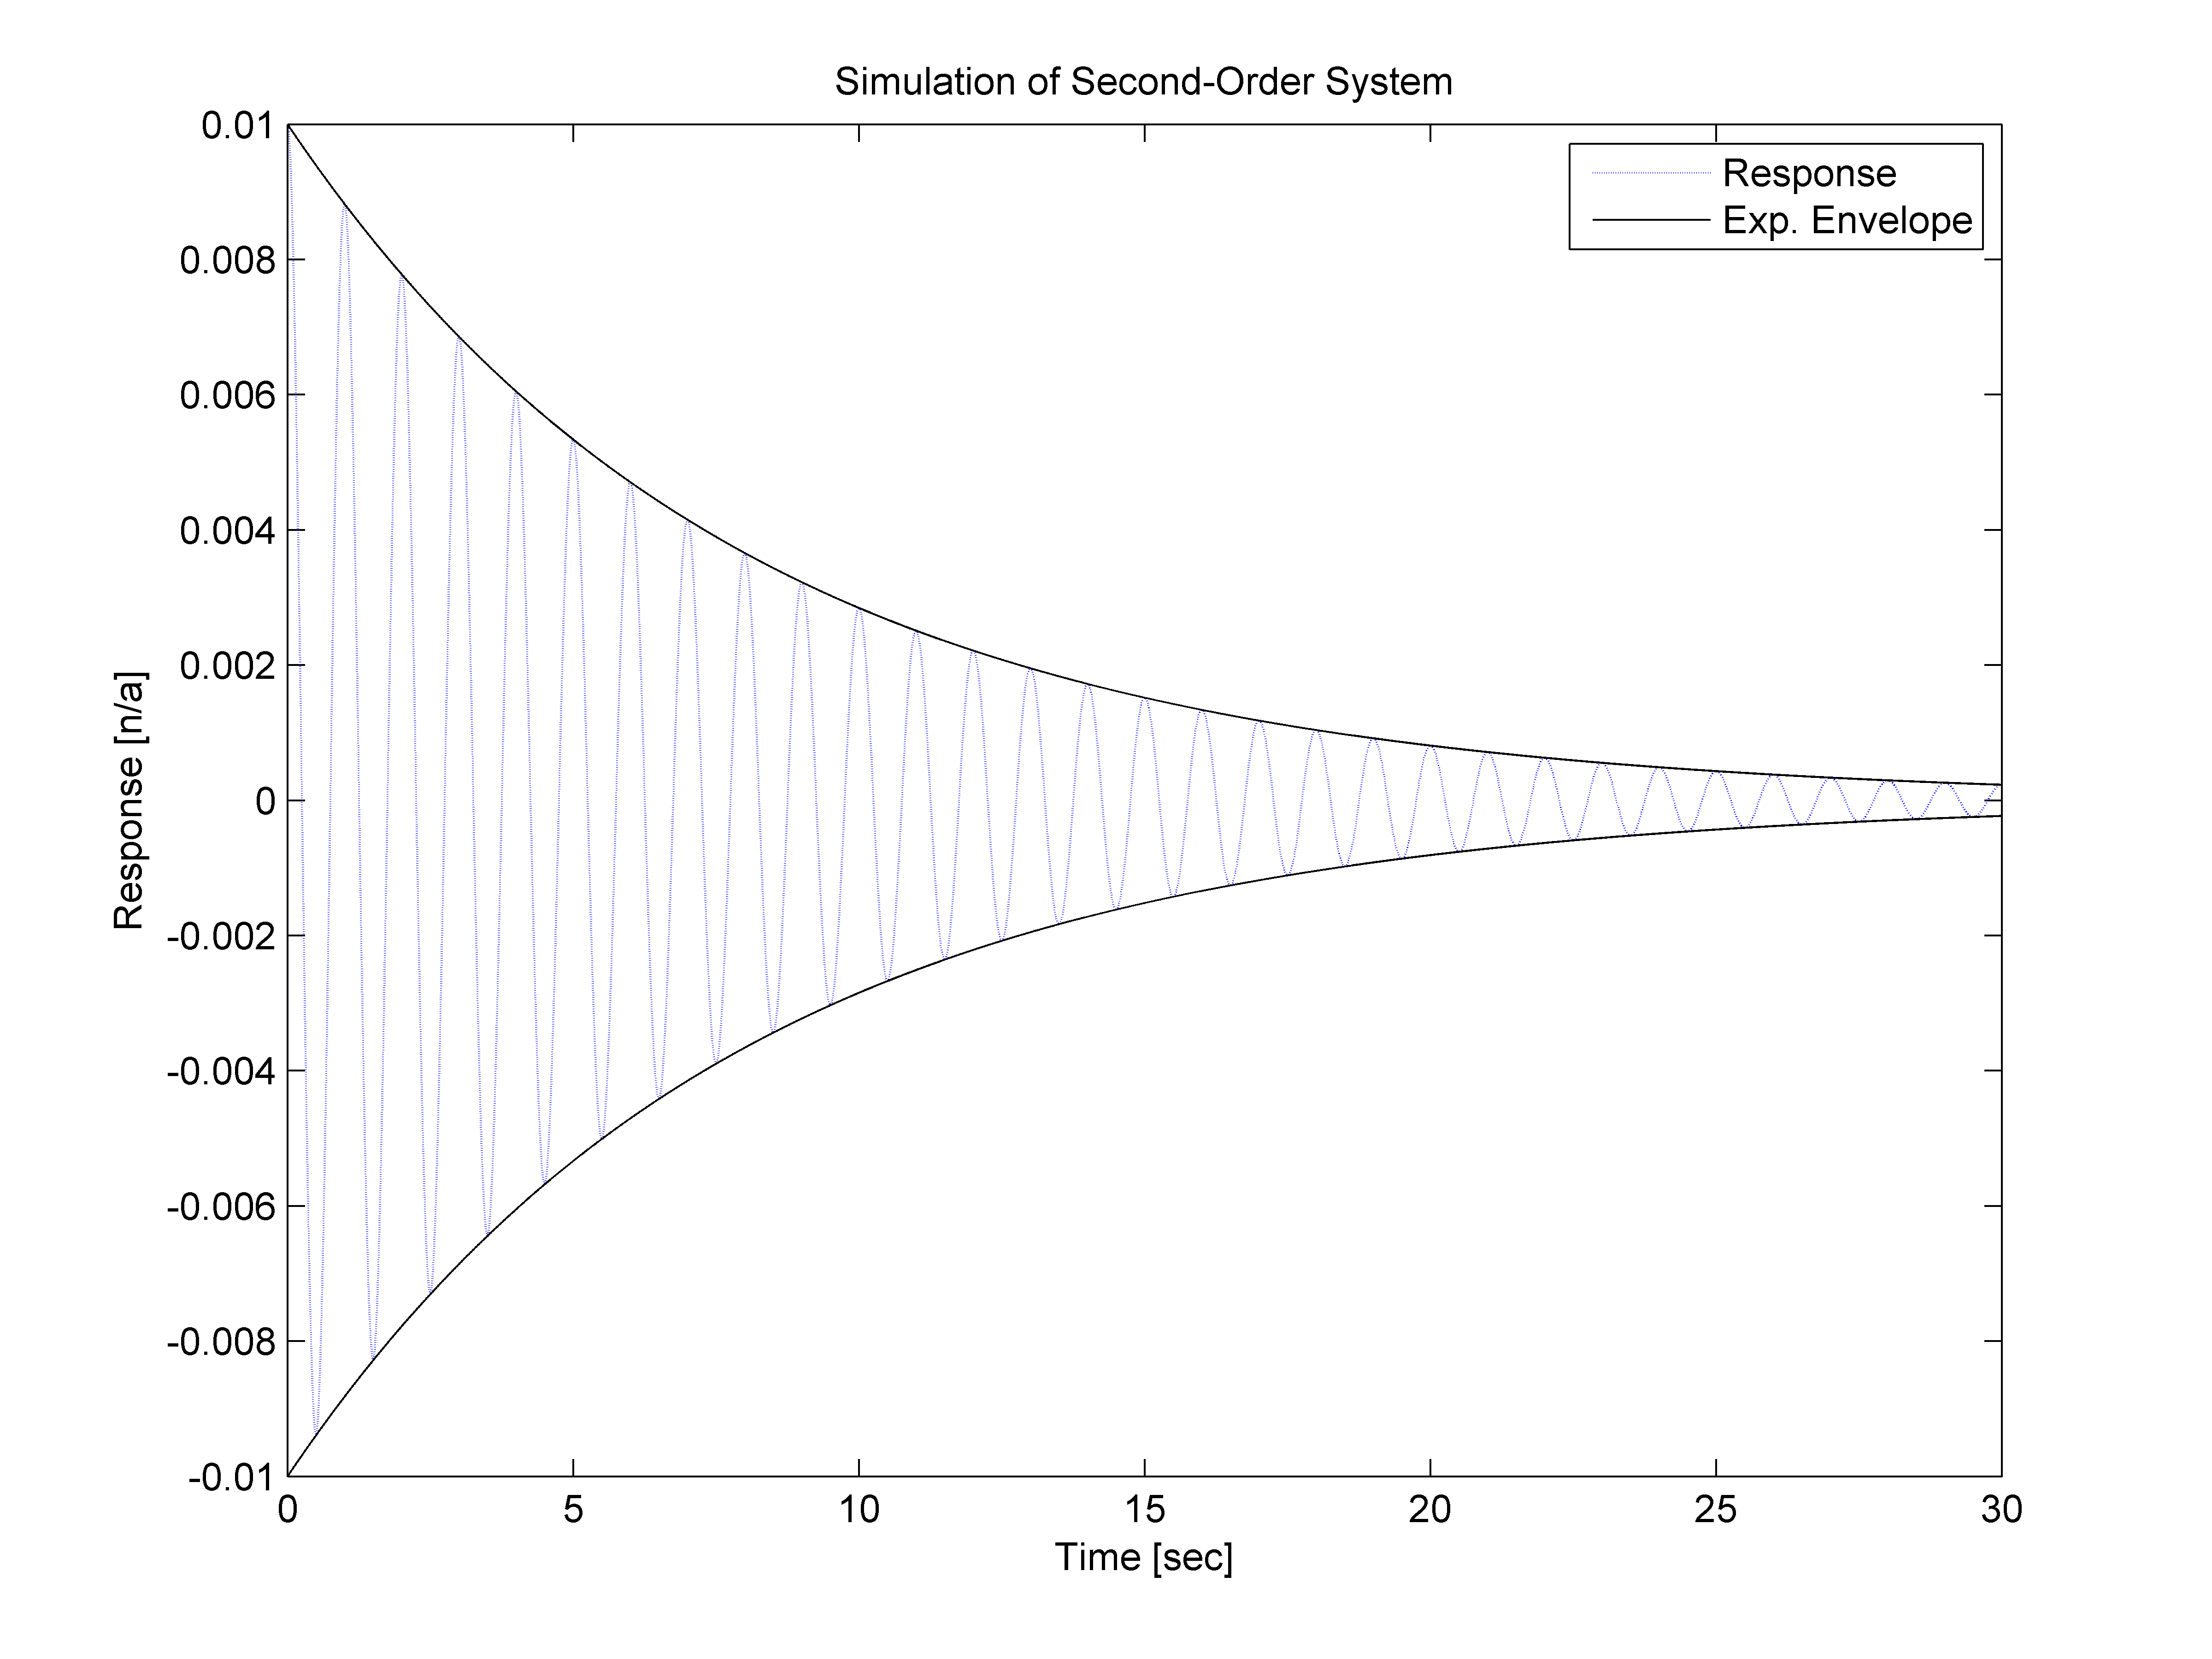
\includegraphics[width=0.6\textwidth]{second_order_env.png}}}
\caption{Second-order free response with the exponential envelope function included (\ref{e:env})}.
\label{f:env}
\end{figure}

If we take the natural logarithm of this function we get a linear relationship between $Y_{ln}=\ln(y_{env})$ and $t$.
\[
Y_{ln}=\ln(y_{env})=(-\zeta \omega_n) t
\]
This linear relationship is illustrated in Figure~\ref{f:ln} where $Y_{ln}$ is plotted versus time.  The slope of the line is $m=-\zeta \omega_n$.
\begin{figure}[hbt!]
\centerline{
{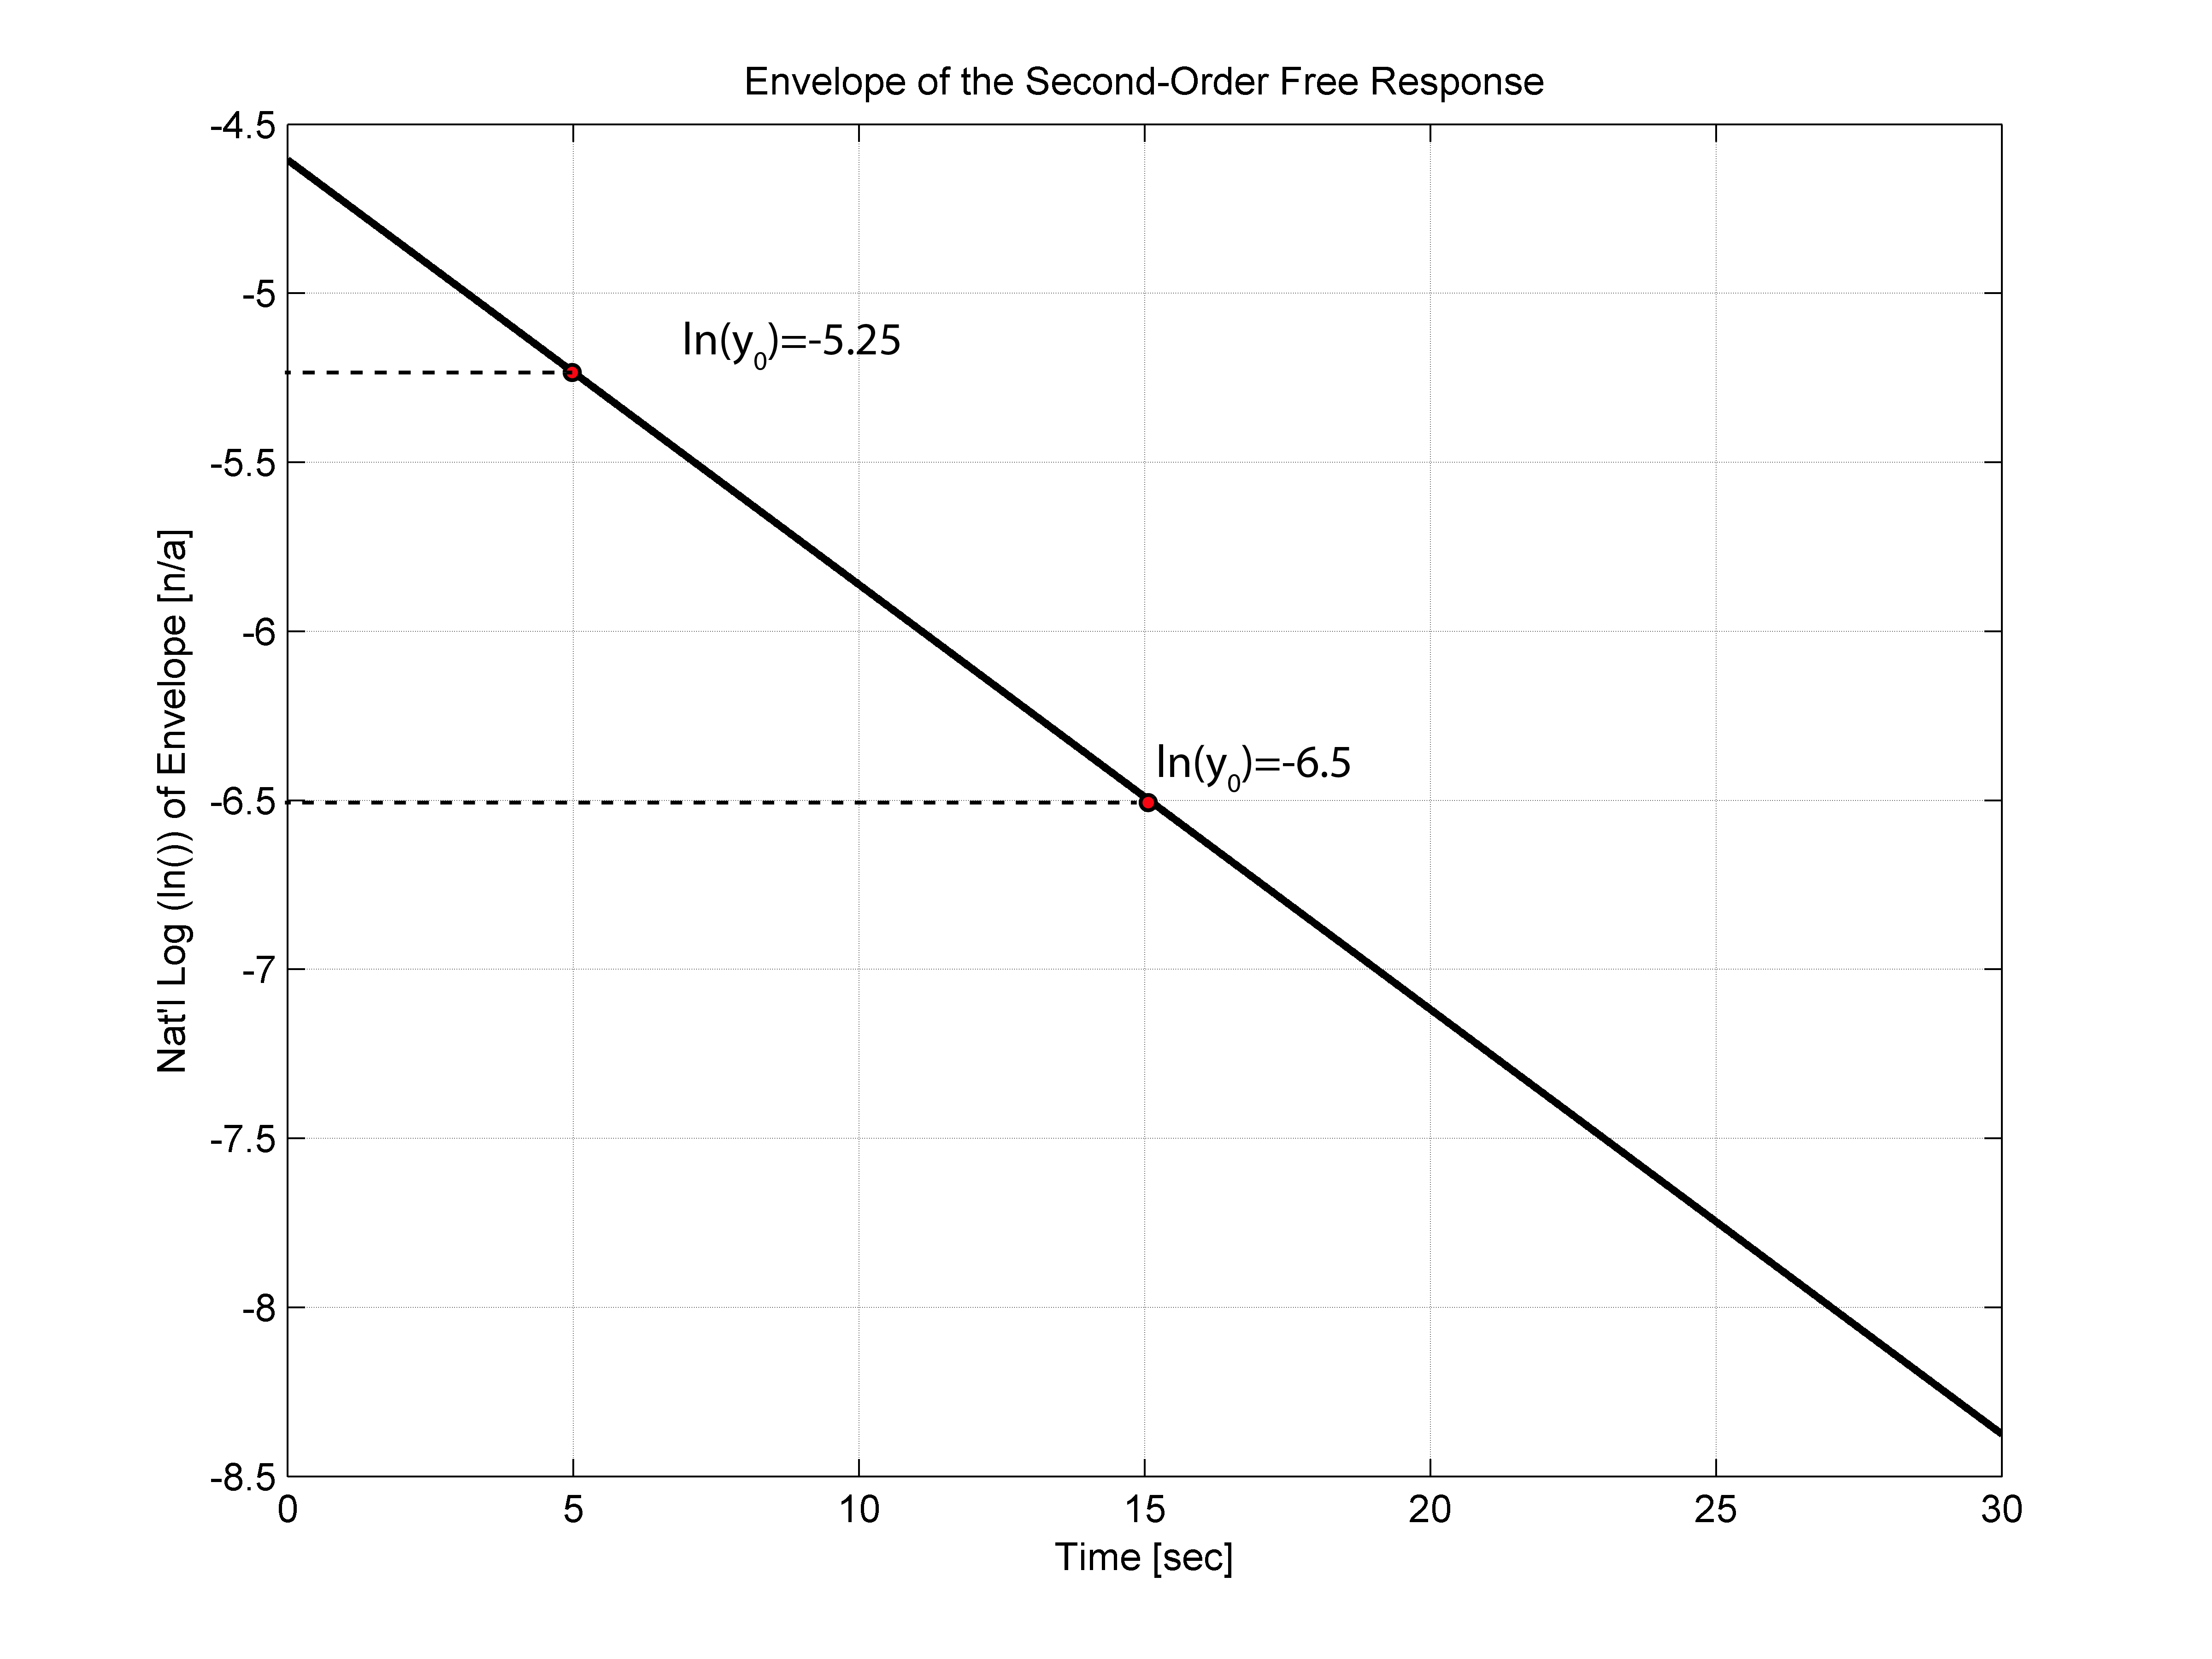
\includegraphics[width=0.6\textwidth]{second_order_env_ln_annote.png}}}
\caption{Plot of the exponential envelope shown in Figure~\ref{f:env}, but here the natural logarithm ($\ln()$) of the amplitude is plotted, i.e., $Y_{ln}$.}
\label{f:ln}
\end{figure}

Because we are using the second-order response model, we now just need to find the slope of the line in Figure~\ref{f:ln} and solve for the damping ratio.  The slope of the line can be expressed as
\begin{eqnarray}
m & = & \frac{\ln(y_0)-\ln(y_n)}{t_0-t_n}=-\zeta \omega_n \\
\label{e:slope} \\
m & = & \frac{\ln(y_0)-\ln(y_n)}{t_n-t_0}=\zeta \omega_n \\
\label{e:slope2}
\end{eqnarray}
We can use (\ref{e:slope}) or (\ref{e:slope2} directly, but we have to deal with the fact that we don't know $\omega_n$.  It is important to note that the frequency of oscillation is the damped natural frequency ($\omega_d$) which is related to the undamped natural frequency by the relationship
\begin{equation}
\omega_d=\omega_n\sqrt{1-\zeta^2}
\label{e:omegas}
\end{equation}
The logarithmic decrement method uses the peaks of the oscillating response to get around this trouble.  We know that the change in time is an integer number of periods of oscillation at the damped natural frequency
\begin{equation}
t_n-t_0 = \frac{n}{\omega_d / 2 \pi}
\label{e:time}
\end{equation}
Now we can substitute (\ref{e:time}) and (\ref{e:omegas}) into (\ref{e:slope2}).
\[
\frac{\ln\left(\frac{y_0}{y_n}\right)}{n (2 \pi)} \omega_d = \zeta \omega_n
\]
\[
\frac{\ln\left(\frac{y_0}{y_n}\right)}{n (2 \pi)} \omega_n \sqrt{1-\zeta^2} = \zeta \omega_n
\]
Let 
\[ \delta = \frac{1}{n}\ln\left(\frac{y_0}{y_n}\right) \]
and we are solve for $\zeta$
\[
\zeta^2=\frac{\left(\frac{\delta}{2 \pi}\right)^2}{1+\left(\frac{\delta}{2 \pi}\right)^2}
\]
\[ \zeta = \frac{1}{\sqrt{1+\left(\frac{2\pi}{\delta}\right)^2}} \]

It is interesting to consider that the logarithmic decrement method is doing this linear-fit with just two data points.  It would be interesting to do this linear fit with multiple data points using a least-squares approach to identify the damping ratio.  One advantage (along with a more precise result) is that you would be able to quantify the ``goodness-of-fit'' for the data using the correlation coefficient ($R^2$).




